\section{Durchführung}
\label{sec:Durchführung}

    Für die Messungen steht ein Lock-In-Verstärker wie in \autoref{fig:gerät} zur Verfügung. Hier sind zur einzelnen Bedienung aller der 
    Komponenten integriert. Oben ist ein Vorverstärker, ein Filter, der als Band-, Hoch- oder Tiefpass benutzt werden kann, und ein 
    Amplituden-/Lock-In-Detektor eingebaut. In der unteren Hälfte ist links ein Noise-Generator, der zur Erzeugung vom Rauschen da
    ist, zu finden. Daneben gibt es einen Generator, den Phasenverschiebung und noch einen expliziten Tiefpass.

    \begin{figure}
        \centering
        \includegraphics[width=0.7\textwidth]{bilder/gerät.png}
        \caption{Der Lock-In-Verstärker. \cite{anleitung}}
        \label{fig:gerät}
    \end{figure}

\subsection{Messung ohne Rauschen}

    Es wird der Lock-In-Verstärker nach der Schaltung in \autoref{fig:schaltung_lockin} aufgebaut, wobei der Noise-Generator überbrückt wird. 
    Es werden im Generator zwei Sinusspannungen mit einer Frequenz von ca $\SI{1}{\kilo\hertz}$ und $\SI{10}{\milli\volt}$ erzeugt. Die 
    Signalfrequenz wird durch den Vorverstärker in den Filter, welcher hier als Bandpass funktioniert, geleitet und schließlich in den 
    Detektor geschickt. Die Referenzspannung geht über den Phasenschieber auch in den Detektor. Der Output aus dem Detektor wird über
    den Tiefpass geleitet und schließlich auf dem Oszilloskop aufgetragen.

    \begin{figure}
        \centering
        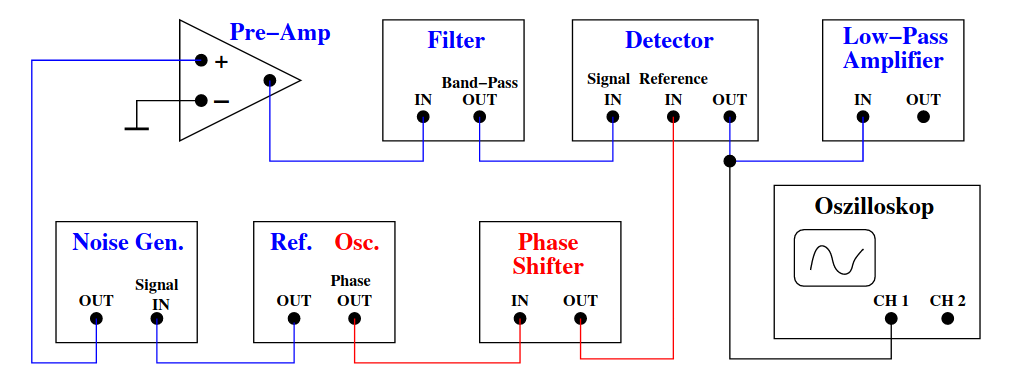
\includegraphics[width=\textwidth]{bilder/schaltkreis_lock_in.png}
        \caption{Der Schaltkreis zur Vermessung einer Sinusspannung mit und ohne Rauschen. \cite{anleitung}}
        \label{fig:schaltung_lockin}
    \end{figure}

    \noindent Nun wird die Phase der Referenzspannung variiert und für verschiedene Phasenlage die Amplitude der Ausgangsspannung gemessen und 
    der Verlauf der Kurve skizziert. 

\subsection{Messung mit Rauschen}

    Hier wird die Schaltung analog zur Messung ohne Rauschen nach der \autoref{fig:schaltung_lockin} aufgebaut. Jetzt wird die sinusförmige 
    Signalspannung durch den Noise-Generator mit Rauschen der gleichen Größenordnung versehen, bevor sie in den Vorverstärker geht. Es ist 
    zu beachten, dass im Noise-Generator auch ein Verstärker verbaut ist. \\
    Es wird wieder die Amplitude der Ausgangsspannung für verschiedene Phasenlage der Referenz- und Signalspannung gemessen und der Verlauf 
    der Kurve skizziert. 

\subsection{Messung mit einer Photodiode}

    Nun wird eine Photodetektorschaltung wie in \autoref{fig:schaltung_diode} aufgebaut. Die Leuchtdiode wird mit einer Rechteckspannung 
    von $\SI{500}{\hertz}$ gespeist. Das Licht wird mit einer Photodiode gemessen, der Output der Diode ist die genutzte Signalspannung.
    Die Leuchtdiode sowie die Photodiode befinden sich auf einer optischen Bank.  
    Die Referenzspannung hat eine Phasenverschiebung von $\SI{360}{\degree}$. Es wird die Amplitude der Ausgangsspannung für verschiedene
    Abstände $r$ zwischen Leucht- und Photodiode gemessen.

    \begin{figure}[H]
        \centering
        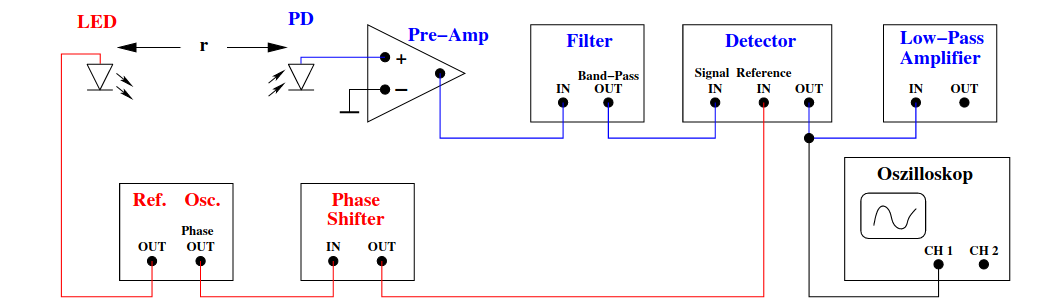
\includegraphics[width=\textwidth]{bilder/schaltkreis_diode.png}
        \caption{Dir Schaltung zur Messung mit einer Photodiode als Signalspannung. \cite{anleitung}}
        \label{fig:schaltung_diode}
    \end{figure}


    \noindent In der \autoref{fig:foto_apparatur} ist der Aufbau des Experimentes von der Messung mit der Sinusspannung mit und ohne
    Rauschen zu sehen. Auf dem Lock-In-Verstärker, welcher dem in \autoref{fig:gerät} gleicht, steht das Oszilloskop.  
    In der \autoref{fig:foto_diode} sind die Photodiode (links) und die Leuchtdiode (rechts) auf einer optischen Bank 
    zu sehen.

    \begin{figure}
        \centering
        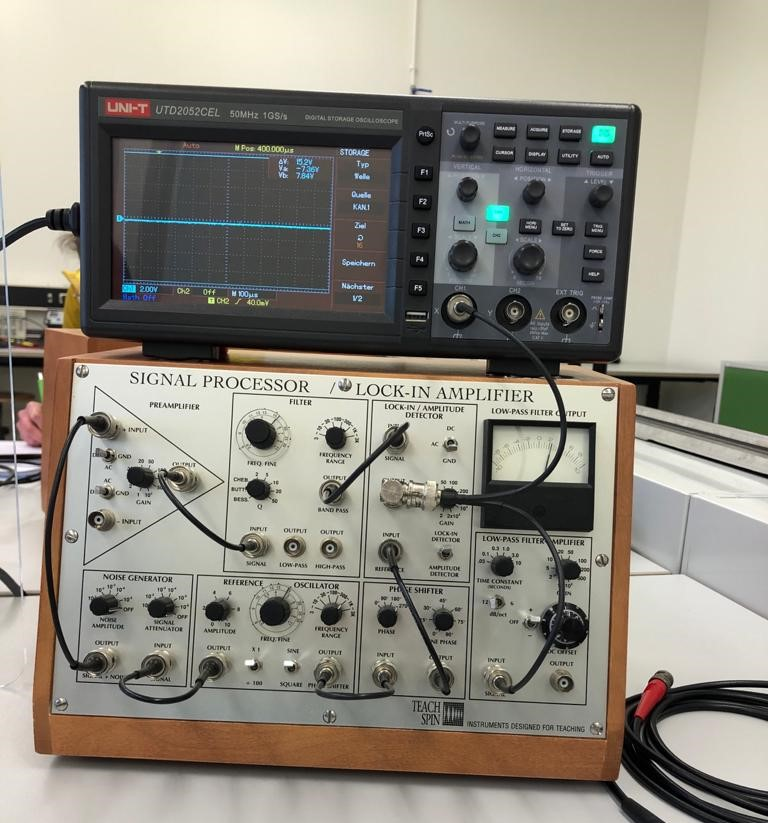
\includegraphics[width=\textwidth]{bilder/foto_apparatur.jpeg}
        \caption{Der Originalaufbau, welcher im Experiment genutzt wird.}
        \label{fig:foto_apparatur}
    \end{figure}

    \begin{figure}
        \centering
        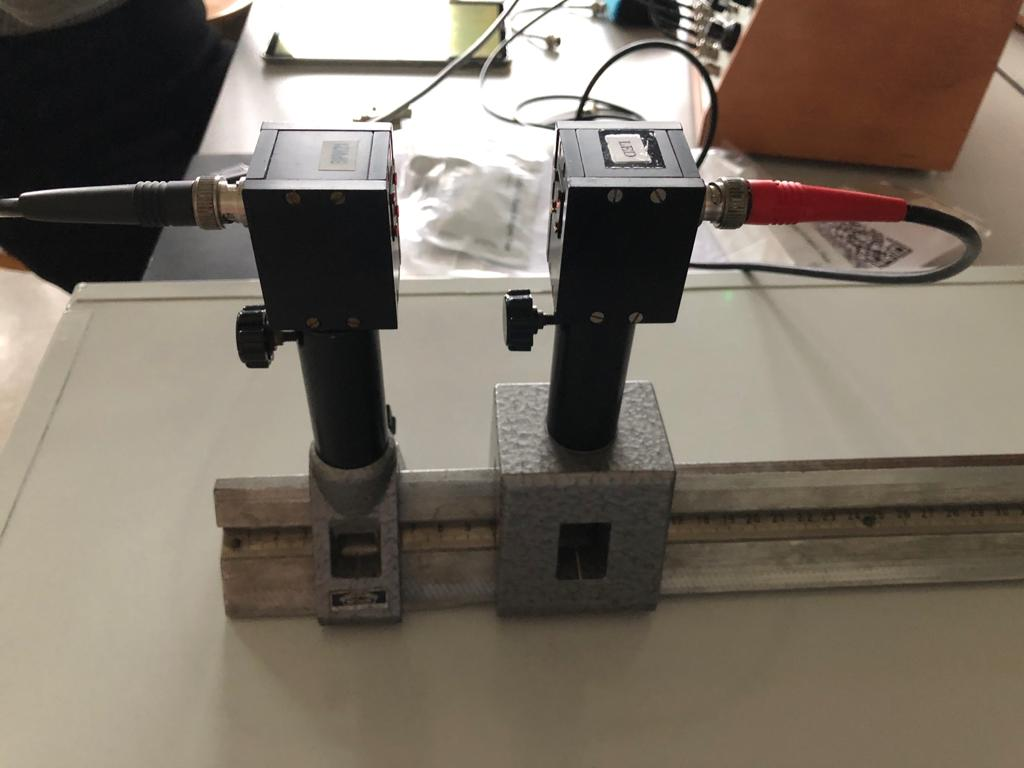
\includegraphics[width=\textwidth]{bilder/foto_diode.jpeg}
        \caption{Die Leucht- und Photodiode auf einer optischen Bank.}
        \label{fig:foto_diode}
    \end{figure}